\chapter{Developed Approaches to Visual Object Tracking}
\label{chap:DevelopedVisualTrackingApproaches}

In this chapter, we dive into our contributions to the field of Siamese-based \gls{vot}. This entire chapter follows a specific pattern. It consists of four sections in total, and every section begins with motivation, then elaborates on some particular solution, and finishes off by providing experimental evaluation followed by a discussion. We start by commenting on why we think the most important tracker, the \gls{siammot} framework, was chosen as a base for our experimentation, and then proceed to a general description of this approach (\sectiontext{}~\ref{sec:SiamMOT}). Subsequently, we propose our first enhancement to this tracker based on top of external neural network used for object \gls{reid} (\sectiontext{}~\ref{sec:SiamMOTandReID}). In the following section, we describe our experiments aimed at incorporating learning metric embeddings into the end-to-end training pipeline of the \gls{siammot} tracker itself (\sectiontext{}~\ref{sec:SiamMOTandFeatureEmb}). We close the chapter by examining the inclusion of attention mechanism and a deformable convolution operation, once again, by altering the end-to-end tracking pipeline (\sectiontext{}~\ref{sec:SiamMOTandAttention}).

\section{Siamese Multi-Object Tracking}
\label{sec:SiamMOT}

This section is dedicated to the most important tracker we have encountered during our research, called \siammot{}~\cite{shuai2021siammot}. Its importance stems from the fact that the majority of our experiments adopted this model. Even though this section could be part of the theoretical foundations chapter, we found it more comprehensible to provide the description of the base architecture closer to the description of our methods and experiments.

% ##############################################################################
\subsection{General Description}

The authors of~\cite{shuai2021siammot} tracker focused on improving online \gls{mot}. As far as their methodology was concerned, they employed region-based approach~\cite{ren2017fasterrcnn} in conjunction with a Siamese multi-object tracking network, hence the name \siammot{}. Broadly speaking, this architecture employes Siamese tracker for motion estimation between two frames. We would like to note that all the principles so far discussed regarding Siamese trackers apply here. However, as already suggested, the adoption of \gls{rpn} enables this framework to have more information available. Not only there is the motion prediction from the Siamese tracker, there are also detections produced by the \fasterrcnn{} object detector~\cite{ren2017fasterrcnn} that is integrated within the whole architecture. Subsequently, an online solver is utilized to merge these prediction obtained from the tracker and detector heads. It is no surprise that such a framework that exploits modern approaches (more on that later) to object detection and Siamese tracking produces \gls{sota} performance.

We will disect this framewrok in great detail since we studied it scrupulously. We performed multiple experiments, many of which did not yield expected improvements. Nevertheless, the practical part of our work was focused on contributing to the open source repository dedicated to this project developed by several Amazon researchers~\cite{websiammotoriggithub}. We followed a standard path of how contributing to open source projects should be done in a transparent and, more importantly, compatible fashion. We initialized a fresh fork of this project on our personal GitHub account~\cite{websiammotforkgithub} to preserve as much compatibility with the original software as possible and to not strip ourselves of the opportunity to easily receive potential updates from the original repository.

During our development we often engaged in discussions related to this project incentivized by other researchers who were also working on this project and trying to either only apply this work to their specific use case or even extend the model. Our detailed knowledge of this model acquired through deliberate and long-lasting work on this project often helped several other programmers who dealt with various issues. From the programming standpoint, our work involved a considerable amount of programming, even though the base architecture was provided and fully functional. We would like to emphasize that the project consisted of $?$ lines of source code programmed purely in Python programming language. Concerning the deep learning aspect, the PyTorch library~\cite{paszke2019pytorch} was primarily used. It is a widely known library aimed at building deep neural network models while exploiting automatic differentiation.

% ##############################################################################
\subsection{Model Architecture}

The two key aspects of the the \siammot{} architecture are \fasterrcnn{}~\cite{ren2017fasterrcnn} object detector and Siamese tracker. The salient element of the \fasterrcnn{} is the \gls{rpn}. Simply put, \siammot{} adds a region-based Siamese tracker along the standard $2$-stage object detection pipeline in order to model instance-level motion.

As depicted in \figstr{}~\ref{fig:SiamMOTArchitecture}, the input consists of two frames, namely $\mtxsup{I}{t}$ and $\mtxsup{I}{t + \delta}$, accompanied by a set of detected object instances $\mtxsup{R}{t} = \cbrackets{\subsup{R}{1}{t}, \subsup{R}{2}{t}, \dots, \subsup{R}{i}{t}, \dots}$ at time $t$. During the inference process, the detection head produces a set of detected object instances $\mtxsup{R}{t + \delta}$ whilst the tracker's task is to propage the detections $\mtxsup{R}{t}$ to time $t + \delta$, and thus yielding the tracker output denoted as $\mtxsup{\tilde{R}}{t + \delta}$. Please note that it is not the output of the entire tracker, only of the Siamese tracker itself. These instances have to be further processed. Explained next.

This framework relies on a motion model that \emph{tracks} each detected object instance from time $t$ to $t + \delta$. A specific \gls{bbox} $\subsup{R}{i}{t}$ at time $t$ is thus propagated to its future counterpart $\subsup{\tilde{R}}{i}{t + \delta}$ at time $t + \delta$. Such a procedure is then completed by a spatial matching process the objective of which is the \emph{association} of the tracker output $\subsup{\tilde{R}}{i}{t + \delta}$ with detections $\subsup{\tilde{R}}{i}{t + \delta}$ at time $t + \delta$ such that detected instances are linked from $t$ to $t + \delta$.

Assume there is a specific object instance $i$ detected at time $t$. Then, the Siamese tracker searches for this particular instance at frame $\mtxsup{I}{t + \delta}$ while exploiting a contextual window spanning a fixed neighborhood of the object's location (i.e., $\subsup{R}{i}{t}$) at frame $\mtxsup{I}{t}$. In order to define this step more formally, consider the following dependency:
\begin{equation}
    \label{eq:SiamMOTSiameseTracker}
    \rbrackets{
        \subsup{v}{i}{t + \delta},
        \subsup{\tilde{R}}{i}{t + \delta}
    } =
    \func{\mathcal{T}}{
        \mtxsubsup{f}{R_i}{t}, \mtxsubsup{f}{S_i}{t + \delta}; \Theta
    },
\end{equation}
where $\mathcal{T}$ is a module (head) represented by the Siamese tracker with learnable parameters $\Theta$. In light of the already stated efficiency of this framework in terms reusing information as much as possible, the module $\mathcal{T}$ is trained on shared feature maps extracted from the backbone using \gls{roi}-align operations. As a short reminder, a basic Siamese tracker uses an exemplar image encoded as a kernel to search for the occurrence of the corresponding object in a future frame over a specific search region that should be, by definition, greater than the exemplar region. Thus, the feature map $\mtxsubsup{f}{R_i}{t}$ is extracted over the region $\subsup{R}{i}{t}$ contained in the frame $\mtxsup{I}{t}$. Analogically, the feature map $\mtxsubsup{f}{S_i}{t + \delta}$ is extracted over the search region $\subsup{S}{i}{t + \delta}$ delineated in the frame $\mtxsup{I}{t + \delta}$. The region $\subsup{S}{i}{t + \delta}$ is computed by simple expansion of the region $\subsup{R}{i}{t}$ by a factor $r$, such that $r > 1$, while preserving the location of the geometric center, as illustrated in \figstr{}~\ref{fig:SiamMOTArchitecture} by the dashed \gls{bbox}. Once again, a standard procedure of region expansion while maintaining the original region in the center of the specified region that is ubiquitous among single-object Siamese trackers. Last but not least, $\subsup{v}{i}{t + \delta}$ represents the visibility confidence for the detected instance $i$ at time $t + \delta$. This visibility score reflects the tracker's prediction confidence, and so the value $\subsup{v}{i}{t + \delta}$ should be high if the instance is visible in $\subsup{S}{i}{t + \delta}$, otherwise the value should be low. On top of this formulation that is reminiscent of single object tracking, in the \gls{mot} context \eqstr{}~\ref{eq:SiamMOTSiameseTracker} is applied multiple times, i.e., for each object detected in frame $t$, signified by $\subsup{R}{i}{t} \in \mtxsup{R}{t}$. However, from implementation's perspective, all these operations can run in parallel and thus the backbone features are computed only once, making the online tracking inference very efficient.

\begin{figure}[t]
    \centering
    \includegraphics[width=\linewidth]{figures/methodology/siammot_architecture.pdf}
    \caption[\siammot{} architecture]{The base architecture of the \siammot{} model. This tracker detects and associates object instances simultaneously. The Siamese tracker situated in the top branch serves the purpose of predicting motion of objects across frames, thus faciliates temporal linking of objects in an online fashion. Simply put, the Siamese tracker module can be thought of as a single object tracker with all the pros and cons we have discussed so far. On the other hand, a $2$-stage object detection is performed as part of the bottom branch. These two branches are then merged using a solver that spatially and temporally attemps to match tracker and detector predictions to produce the tracker output. We have to emphasize that the spatial matching and solver blocks are only used during the inference and are not differentiable. Note that the feature map corresponding to the frame $\mtxsup{I}{t}$ is shrunk to $\nicefrac{1}{2}$ of its actual size to fit the figure. Backbone features are identical in terms of tensor shapes for both inputs. \externalsrc{\cite{shuai2021siammot}}}
    \label{fig:SiamMOTArchitecture}
\end{figure}

The authors conjectured that motion modeling is of paramount importance for online \gls{mot}. Given our experience in this field so far, we agree. The motion modeling is practically reponsible for association between $\mtxsup{R}{t}$ and $\mtxsup{R}{t + \delta}$. Despite its efficacy, there are still issues to be addressed. The association will fail due to the following reasons:
\begin{enumerate}
    \item if $\mtxsup{\tilde{R}}{t + \delta}$ does not match to the correct object instance in $\mtxsup{R}{t + \delta}$,
    \item or if $\subsup{v}{i}{t + \delta}$ is low (below a specific threshold) for a visible object (person, vehicle, etc.) at time $t + \delta$.
\end{enumerate}
In order to tackle the problems outlined above, the Siamese tracker exploits various \gls{sota} techniques developed in the single-object Siamese tracking community. We affirmatively approve of the authors decisions, since we deliberately elaborated on multiple aspects that this tracker heavily relies upon in our survey on Siamese tracking~\cite{ondrasovic2021siamese}.

As far as the Siamese part of the \siammot{} is concerned, the authors dubbed their technique as ``explicit motion modeling''. They also worked with ``implicit motion modeling'', but that branch of experiments was neither sufficiently expanded in the paper nor it is of particular importance for our research due to its inferior performance. It only servered the purpose of having a baseline to overcome during evaluation.

\subsubsection{Explicit Motion Modeling}

The most fundamental aspect of Siamese trackers is the cross-correlation operator (\sectionstr{}~\ref{}) to generate a pixel-level $2$D response map. In \siammot{}, this operation correlation each location of the search feature map (belonging to the search region) $\mtxsubsup{f}{S_i}{t + \delta}$ with the exemplar (target) feature map $\mtxsubsup{f}{R_i}{t}$ to produce a response map
\begin{equation}
    \mtxsub{r}{i} = \mtxsubsup{f}{S_i}{t + \delta} \star \mtxsubsup{f}{R_i}{t}.
\end{equation}
Therefore, each map $r_i$ captures a different aspect of similarity at every pixel.

Inspired by the \gls{fcos}~\cite{tian2019fcos} visual object detector, this tracker adopts fully-convolutional network $\psi$ to facilitate instance detection using the response map $\mtxsub{r}{i}$. Besides, the so-called ``centerness'' is also utilized in this architecture (discussed later). The network $\psi$ enables a prediction of a dense visibility confidence map $\mtxsub{v}{i}$. Every pixel of $\mtxsub{v}{i}$ is used as an indicator of the likelihood that this pixels falls within the location of the target object. Besides, a dense location map $\mtxsub{p}{i}$ is also predicted with the goal of encoding offsets from that particular location to the top-left and bottom right \gls{bbox} corners. Consequently, the instance region at $\rbrackets{x, y}$ can be derived by the transformation
\begin{equation}
    \func{\mathcal{R}}{\func{\mtx{p}}{x, y}} =
    \sbrackets{x - l, y - t, x + r, y + b},
\end{equation}
where $\func{\mtx{p}}{x, y} = \sbrackets{l, t, r, b}$, i.e., individual corner offsets. This map is then decoded as
\begin{equation}
    \begin{aligned}
                            & \subsup{\tilde{R}}{i}{t + \delta} =
        \func{\mathcal{R}}{\func{\mtxsub{p}{i}}{x^*, y^*}}                                                                      \\
                            & \subsup{v}{i}{t + \delta} = \func{\mtxsub{v}{i}}{x^*, y^*}                                        \\
        \text{s. t. } \quad & \rbrackets{x^*, y^*} = \underset{x, y}{\argmax} \rbrackets{\mtxsub{v}{i} \odot \mtxsub{\eta}{i}},
    \end{aligned}
\end{equation}
in which $\odot$ symbolizes the element-wise multiplication, $\mtxsub{\eta}{i}$ incurs a non-negative penalty score throughout the entire candidate region computed as
\begin{equation}
    \func{\mtxsub{\eta}{i}}{x, y} =
    \lambda \mathcal{C} +
    \rbrackets{1 - \lambda} \func{\mathcal{S}}{
        \func{\mathcal{R}}{
            \func{\mtx{p}}{x, y}
        },
        \subsup{R}{i}{t}
    }.
\end{equation}
Here, the letter $\lambda$, such that $0 \leq \lambda \leq 1$, is a weighting coefficient, $\mathcal{C}$ is the cosine-window function (\sectionstr{}~\ref{}) with respect to the geometric center of the previous target location given by $\subsup{R}{i}{t}$, and $\mathcal{S}$ is a Gaussian function that is supposed to penalize the height-to-width ratio changes between candidate region $\func{\mtx{p}}{x, y}$ and $\subsup{R}{i}{t}$. The aim of the penalty map is to discourage abrupt changes in target location between individual frames during the course of tracking. This technique is widely adopted in Siamese trackers.

\subsubsection{Loss Function}

The loss function for this model consists of multiple parts and for its completeness it requires a triplet $\rbrackets{\subsup{R}{i}{t}, \subsup{S}{i}{t + \delta}, \subsup{R}{i}{t + \delta}}$. The following function is minimized during the training phase:
\begin{equation}
    \begin{aligned}
        \lossf =
         & \sum_{\forall \rbrackets{x, y}}
        \func{l_{\text{focal}}}{
            \func{\mtxsub{v}{i}}{
                x, y
            },
            \func{\mtxsubsup{v}{i}{*}}{
                x, y
            }
        } +                                \\
         & \sum_{\forall \rbrackets{x, y}}
        \mathbbm{1}
        \sbrackets{
            \func{\mtxsubsup{v}{i}{*}}{
                x, y
            } = 1
        }
        \rbrackets{
            \func{w}{x, y}
            \cdot
            \func{l_{\text{reg}}}{
                \func{\mtxsub{p}{i}}{x, y},
                \func{\mtxsubsup{p}{i}{*}}{x, y}
            }
        }
    \end{aligned}.
\end{equation}
In the expression above, the pairs $\rbrackets{x, y}$ enumerate all valid position within the $\subsup{S}{i}{t + \delta}$ region. The loss function dedicated to regression task, i.e., $l_{\text{reg}}$, is formulated as the \gls{iou} loss for regression~\cite{danelljan2019atom, yu2016unitbox}. To address the class-balance problem in an effective way, the focal loss for classification~\cite{lin2018focal} given by the term $l_{\text{focal}}$ is employed, too. All ground-truth values are marked by the $*$ character. So,
\begin{equation}
    \func{\mtxsubsup{v}{i}{*}}{x, y} =
    \begin{cases}
        \begin{aligned}
             & 1 & \text{if } \rbrackets{x, y} \text{ is within } \subsup{R}{i}{*, t + \delta} \\
             & 0 & \text{otherwise}                                                            \\
        \end{aligned}
    \end{cases},
\end{equation}
and
\begin{equation}
    \func{\mtxsubsup{p}{i}{*}}{x, y} =
    \sbrackets{
        x - \subsup{x}{0}{*},
        y - \subsup{y}{0}{*},
        \subsup{x}{1}{*} - x,
        \subsup{y}{1}{*} - y
    },
\end{equation}
where $\rbrackets{\subsup{x}{0}{*}, \subsup{y}{0}{*}}$ and $\rbrackets{\subsup{x}{1}{*}, \subsup{y}{1}{*}}$ correspond to the top-left and bottom-right coordinates of the ground-truth \gls{bbox} $\subsup{R}{i}{t + \delta}$, respectively. Following the line of inspiration from the \gls{fcos}~\cite{tian2019fcos} tracker, the regression loss $l_{\text{reg}}$ is additionally modulated by computing the ``centerness'' for every location (see \figstr{}~\ref{fig:FCOSCenterness}). This concept describes the amount of deviation of the pixel's location from the object center. The reason for adding this score was to suppress locations that are further away from the object's center, because they produced low-quality \gls{bbox} predictions. This score is then used as a weighting. The ``centerness'' coefficient $\func{w}{x, y}$ is calculated for each pixel with respect to the target instance $\subsup{R}{i}{t + \delta}$ as
\begin{equation}
    \label{eq:Centerness}
    \func{w}{x, y} =
    \sqrt{
        \frac{\minf{x - x_0, x_1 - x}}{\maxf{x - x_0, x_1 - x}}
        \cdot
        \frac{\minf{y - y_0, y_1 - y}}{\maxf{y - y_0, y_1 - y}}
    }.
\end{equation}

\begin{figure}[t]
    \centerline{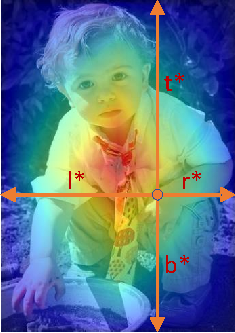
\includegraphics[width=0.2\linewidth]{figures/methodology/fcos_centerness.pdf}}
    \caption[Centerness visualization]{Red, blue, and other colors denote $1$, $0$ and the values between them, respectively. Centerness is calculated as given by \eqstr{}~\ref{eq:Centerness} and decays from $1$ to $0$ as the location deviates from the center of the object. Best viewed in color. \externalsrc{\cite{tian2019fcos}}}
    \label{fig:FCOSCenterness}
\end{figure}

% ##############################################################################
\subsection{Training and Inference Phases}

The \siammot{} model can be trained in an end-to-end fashion, which is one of its great advantages in terms of usability, among others. The general loss function can be formulated as
\begin{equation}
    \label{eq:SiamMOTGeneralLoss}
    \lossf = l_{\text{rpn}} + l_{\text{detect}} + l_{\text{motion}},
\end{equation}
where the $l_{\text{rpn}}$ as well as the $l_{\text{detect}}$ are standard \gls{rpn}~\cite{ren2017fasterrcnn} and detection-subnetwork~\cite{girshick2015fast} losses, respectively. The $l_{\text{motion}}$ loss is used to train the Siamese tracker.

For better understanding, we suggest the reader follow the diagram in \figstr{}~\ref{fig:SiamMOTInference}. At inference, the well-established \gls{iou}-based \gls{nms} operation (\sectionstr{}~\ref{ssec:NonMaximumSuppression} is exploited to process the outputs of the detection and tracker subnetwork independently. The subsequent process aimed at spatial-matching is used to merge detections with the tracker output. This stage also involves the already mentioned \gls{iou}-based \gls{nms} operation (thus, in total, it is used three times during the inference).

\begin{figure}[t]
    \centering
    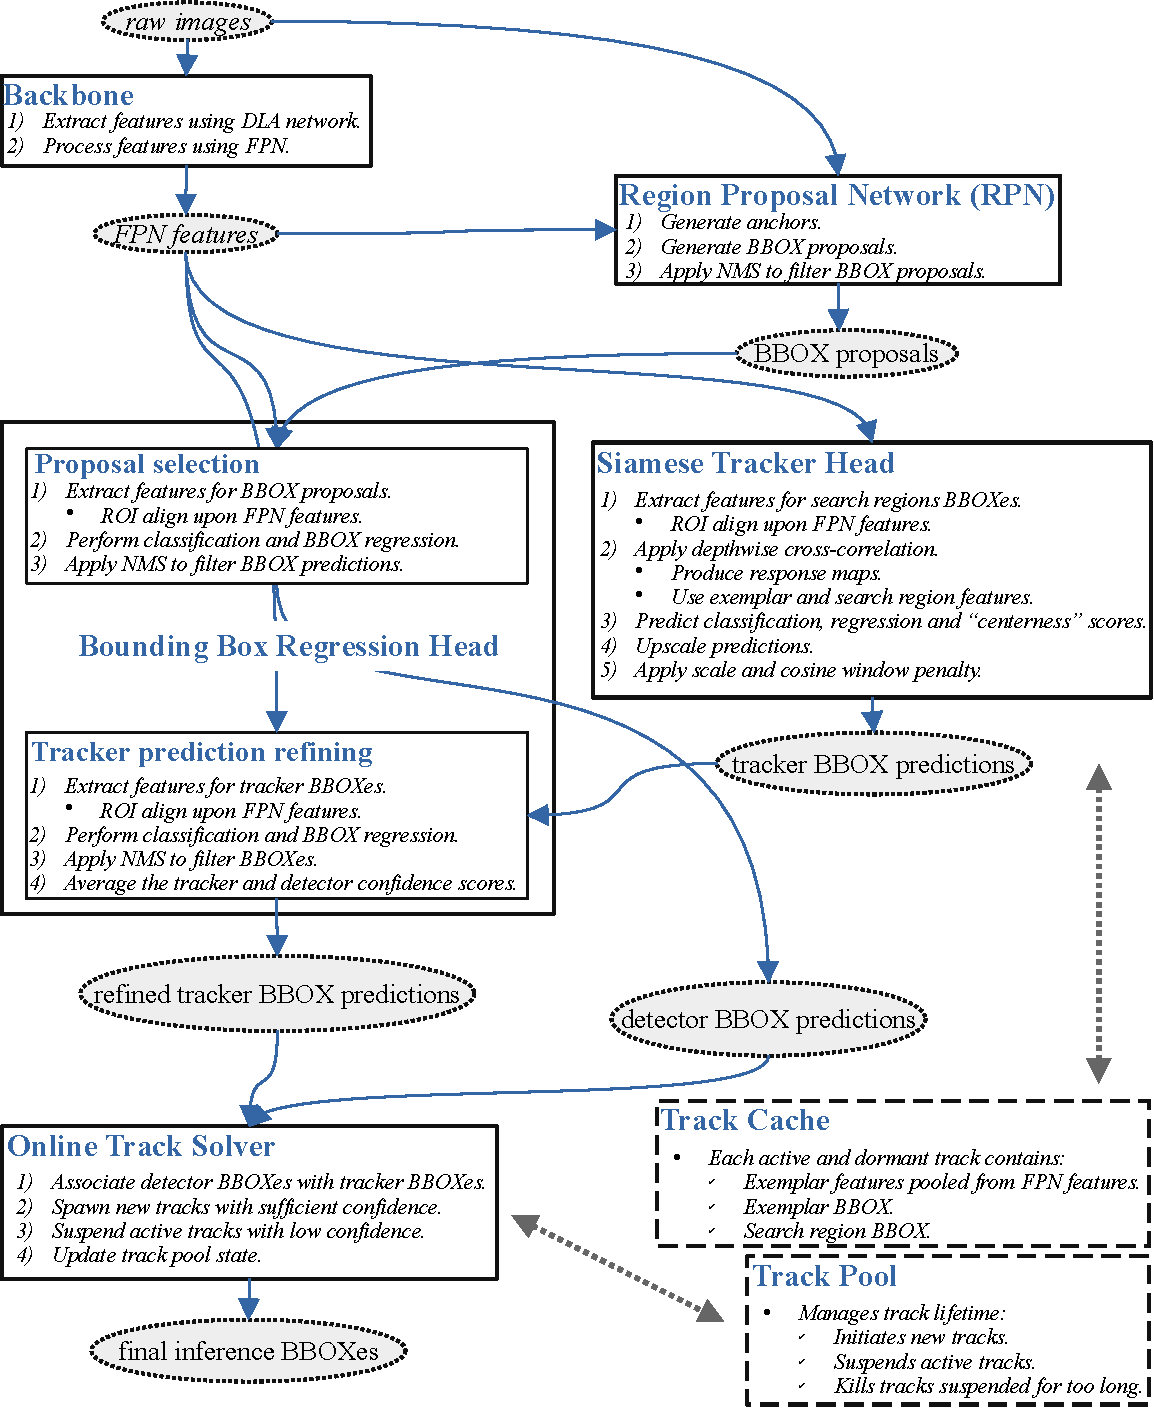
\includegraphics[width=\linewidth]{figures/methodology/siammot_inference_diagram.pdf}
    \caption[\siammot{} inference diagram]{Visualization of the inference pipeline in the \siammot{} architecture. The entire framework efficiently reuses as much information as possible, making it fast and accurate. Backbone features that are a result of intricate \gls{dla} and \gls{fpn} processing are fed into detector and the tracker. Please note that the predictions from the tracker are once again refined using the detector head. Two two aforementioned heads function on top of backbone features through the lens of \gls{roi} align operations. During the inference phase, the ``online solver'' works only with the final \glspl{bbox} produced by the tracker and the object detector. It utilizes a simple caching mechanism to store the backbone features belonging to active or dormant objects. The decision making regarding initialization, suspension and complete removal of track is performed within the ``track pool'' module.}
    \label{fig:SiamMOTInference}
\end{figure}

The spatial-maching is followed by a standard \emph{online} solver that has been widely adopted in numerous works, such as~\cite{bawley2016simple, wojke2017simple, zhou2020tracking, bergmann2019tracking}. In its essence, this solver is simple yet very effective. As our experiments will later demonstrate, it is exceedingly difficult to surpass its performance in general by a significant margin. This solver is governed by the following rules listed below. Let $\subsup{v}{i}{t}$ be the visibility confidence, then
\begin{enumerate}
    \item the object's trajectory is continued as long as its visibility confidence is above a specific threshold $\alpha$, otherwise this trajecotry becomes dormant,
    \item a new trajectory is spawned in case there is a non-matched detection (during the spatial-matching process) and its visibility confidence is above a threshold $\beta$,
    \item a dormant trajectory is terminated, i.e., the object ID will never be used once again, it its visibility confidence is below $\alpha$ for $\tau$ consecutive frames.
\end{enumerate}

\subsubsection{Short-term Occlusion Handling}

This model also attempts to tackle short-term occlusion. It is one of the key incentives that led us to consider this architecture for our experiments, which is the model's ability to handle occlusion in an efficient and trivial manner. At the beginning, we guessed that this phase could be improved upon due to its inherent simplicity. However, regardless of how rudimentary their approach may seem, it implicitly addresses a great deal of frequent cases that apprear in object tracking in a competent way. Our endeavors later described often involved a minor improvement in rare situations with simultaneous minor detriments to common situations. Therefore, the outcome of perfoming worse than the baseline on average was usually inescapable.

A short-term occlusion can be defined as having the visibility confidence for the currently tracker object below the threshold $\alpha$. In \siammot{}, instead of definitely ceaseing the track's existence, the relevant information are kept in memory and thus the search for the exemplar continued until $\tau > 1$ frames have been processed in hope of re-instatiating the object. The most recently predicted location and its corresponding feature frames extracted from the backbone are utilized as the searching template.

\subsubsection{Online Solver Algorithm}

% ##############################################################################
\subsection{Implementation Details}

The \siammot{} model is a paragon of feature pooling.

% ##############################################################################
\subsection{Relevant Implementation-Related Remarks}

In this short section, we would like to summarize several relevant remarks related to the \siammot{} model.

\subsubsection{Pre-training}

Overall, the model is not difficult to train. By difficult training we mainly mean instability and sensitivity to hyperparameters. However, the training itself requires a great deal of GPU VRAM available in order to use sufficiently large minibatches. As far as our development experience with the \siammot{} model is concerned, we used the \texttt{NVidia}~\cite{webnvidia} \texttt{RTX 2080Ti} graphics cards which provides $4352$ CUDA cores together with $11$GB of GDDR6 memory. For traning, we often exploited an existing backbone model pre-trained on ImageNet~\cite{deng2009imagenet} dataset provided by the authors. Even though there is the entire model available pre-trained on \mscoco{}~\cite{lin2014mscoco} dataset, we decided to avoid it due to conflicting nature of object classes. We observed better performance when training vehicle detection from scratch rather than trying to ``re-wire'' the model to dismiss detecting objects we wanted to avoid in the first place, e.g., pedestrians.

\subsubsection{Gradient Accumulation}

Since majority of our experiments involved expanding the model by adding additional heads, we often struggled with the amount of available GPU VRAM in order to preserve reasonable size of minibatches. To this end, we also experimented with gradient accumulation. This technique allows the user to postpone the model weight updating after more minibatches have been processed. Therefore, the programmer may simulate using larger minibatches than actually are utilized. We emphasize the importance of not updating the model variables must during the accumulation phase so as to to ensure that all the mini-batches are processed by the same model variable values to calculate their gradients. Only after accumulating the gradients of the values of the model weights can be adjusted accordingly.

For a brief illustration, let $w$ be a single weight we want to update with respect to the computed gradient using the loss function $f$. Our goal is to adjust the weight at time $t$ and thus produce the weight at time $t + 1$. The learning rate is denoted by $\alpha$. So, the gradient update is usually performed as
\begin{equation}
    w^{t + 1} = w^t - \alpha \nabla \func{f}{w^t}.
\end{equation}
When using gradient accumulation, the update step is modified as
\begin{equation}
    w^{t + 1} = w^t - \alpha \sum_{i = 1}^{n} \nabla \func{f}{w^t}_i,
\end{equation}
where $n$ is the number of accumulated minibatches.

\begin{figure}[t]
    \centering
    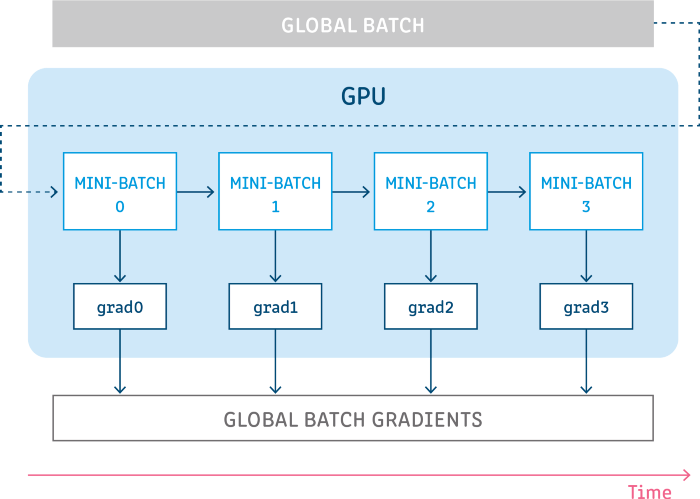
\includegraphics[width=0.6\linewidth]{figures/methodology/gradient_accumulation.png}
    \caption[Gradient accumulation]{Gradient accumulation is a mechanism that allows splitting the minibatch of samples — used for training a neural network — into several even smaller mini-batches of samples that will be processed sequentially. \externalsrc{\cite{webgradaccumulation}}}
    \label{fig:GradientAccumulation}
\end{figure}

Considering the advantages outlined above, it is necessary to acknowledge the potential drawbacks. For example, if batch normalization~\cite{ioffe2015batchnorm} layers are used within the model, then the use of gradient accumulation may possibly have a detrimental effect upon their performance. The reason is that batch normalization layers compute the statistics with respect to a single minibatch. These layers, in their standard formulation and commonly adopted implementation, are incapable of accomodating their innerworkings to adequately administer multiple sequential minibatches. However, there is ongoing research in the direction of group normalization as well, namely works of~\cite{wu2018groupnorm}~and~\cite{zhou2020batchgroupnorm}.

% ##############################################################################
\subsection{Experimental Analysis}
\section{Siamese Multi-Object Tracking and ReID}
\label{sec:SiamMOTandReID}

% ##############################################################################
\subsection{Motivation}

The use of \gls{reid} has been emphasized numerous times during our preliminary research for this thesis. We conjectured that once full occlusion ensues, the \gls{reid} mechanism could be adopted to recover the lost track since the object appears at the scene as a new one. The presence of occlusion percolates traffic scenes, especially if the camera does not view the road from a higher position. At the beginning of our Ph.D. research, we worked on the \interreg{} project where we tackled vehicle tracking when the camera was positioned next to the road (\figtext{}~\ref{fig:InterregDatasetSample}). Under these circumstances, occlusion was inevitable. Such a setup inexorably led to situations in which a vehicle appeared for a second on the left side of the frame, then ended up fully covered by a truck, and re-appeared for a miniscule amount of time at the other side of frame. The task of maintaining the same object identifier was burdensome and often impossible with high degree of precision.

% ##############################################################################
\subsection{Preliminary Discussion}

To make a full disclosure right at the beginning, we expected that the adoption of \gls{reid} enhancements within the \gls{siammot} framework would bring improvements in certain areas. Retrospectively, our experiments showed detrimental effects upon the tracker accuracy. Despite our negative outcome, we still consider the performed research to be a contribution to the \gls{mot} area. We will elaborate further on why it is so in order to learn from such an experience as much as possible. Our surprise stems primarily from the fact that our thesis goals revolved around the application of \gls{reid} in object tracking. Therefore, finding that such approach does not yield the desired outcome raises multiple questions, specifically the following ones:
\begin{enumerate}
    \item Does the inclusion of \gls{reid} into \gls{mot} frameworks have a potential to resolve cases of full occlusion without exacerbating other areas?
    \item Is the \gls{reid} extension suitable to the chosen \gls{mot} model, namely, the \gls{siammot}?
    \item Is the target use case in terms of datasets adequate to showcase the potential of \gls{reid} applied in the \gls{siammot} tracker?
\end{enumerate}

% ##############################################################################
\subsection{Proposed ReID-Enhanced Architecture}
\label{ssec:ProposedReIDEnhancedArchitecture}

We adopted the object \gls{reid} approach published in~\cite{luo2019bagoftricksreid}, a simple yet very robust framework for person \gls{reid}. We employed this architecture (\figtext{}~\ref{fig:BagOfTricksReIDArchitecture}) for vehicle \gls{reid} due to its simplicity accompanied with \gls{sota} performance at the time of publishing.

% ------------------------------------------------------------------------------
\begin{figure}[!t]
    \centering
    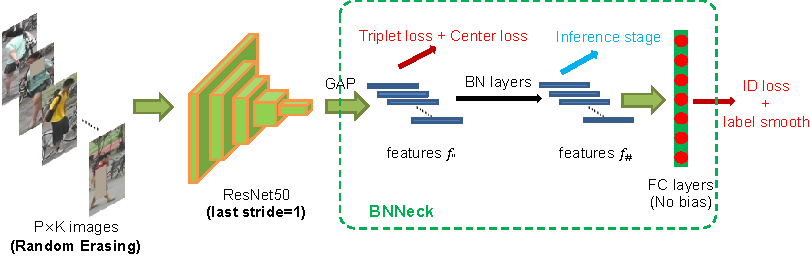
\includegraphics[width=\linewidth]{figures/siamese_tracking/bagoftricks_reid_architecture.pdf}
    \caption[Gls{reid} baseline]{A object \gls{reid} baseline which we used for our experiments. \externalsrc{\cite{luo2019bagoftricksreid}}}
    \label{fig:BagOfTricksReIDArchitecture}
\end{figure}
% ------------------------------------------------------------------------------

% ##############################################################################
\subsection{Training Phase}

% ##############################################################################
\subsection{Inference Phase}

The online solver algorithm was, from our point of view, the primary suspect for potential improvements due to its inherent simplicity that we considered inferior compared to the rest of the architecture.

% ##############################################################################
\subsection{Experimental Evaluation}

% ##############################################################################
\subsection{Discussion}
\section{Siamese Multi-Object Tracking and Embedding}
\label{sec:SiamMOTandFeatureEmb}

% ##############################################################################
\subsection{Motivation}

One of our experiments involved an end-to-end training of the \gls{siammot} model together with a custom head aimed at embeddings based on \gls{roi}-pooled backbone-extracted features for the object \gls{bbox}. The goal was to force the training process into extracting features that are not only satisfactory for detection and tracking but also contain the necessary information to create embeddings for \gls{reid} purposes during the inference.

We strived for simplicity by extending the processing pipeline without altering the existing infrastructure. From the standpoint of implementation, the \gls{siammot} project itself is organized in a proper object-oriented and modular fashion, which made this particular development task easy in this aspect. However, as we will discuss further, we encountered setbacks in terms of training stability and we had to take appropriate measures. Furthermore, extending a huge model that already requires a significant amount of \gls{gpu} \gls{vram} made it even more demanding.

During the research related to our Siamese tracking survey~\cite{ondrasovic2021siamese}, we noticed one work where the exemplar features were projected using \gls{gap} operation into an embedding space consisting of fewer dimensions~\cite{li2020figsiam}. The embedding vector was produced using the feature tensor that represented the kernel for the cross-correlation operation utilized by the majority of the Siamese trackers discussed so far.

More concretely, suppose the extracted features were represented by a tensor of shape $8 \times 8 \times 256$. Then, the \gls{gap} operation along the channel dimension would produce a tensor of shape $1 \times 1 \times 256$, which could then be further flattened into a single $256$-dimensional vector. In the end, the obtained vector was $l_2$-normalized and thus projected onto a unit hypersphere. In the work of Li~\etal{}~\cite{li2020figsiam}, these embedding vectors were exploited for template updating and for combining multiple templates within a pool of size $n$ in an exponential fashion.

This observation led us to the following hypothesis. Given the fact the Siamese exemplar features do contain some, although probably not sufficient information for pure object \gls{reid}, would it be possible to map them further using a non-linear function to produce embedding vectors that could serve for \gls{reid}? Such features are just a learned template, therefore, some notion of similarity needs to be already built into it.

% ##############################################################################
\subsection{Feature Embedding Head Architecture}

% ------------------------------------------------------------------------------
\begin{figure}[!t]
    \centering
    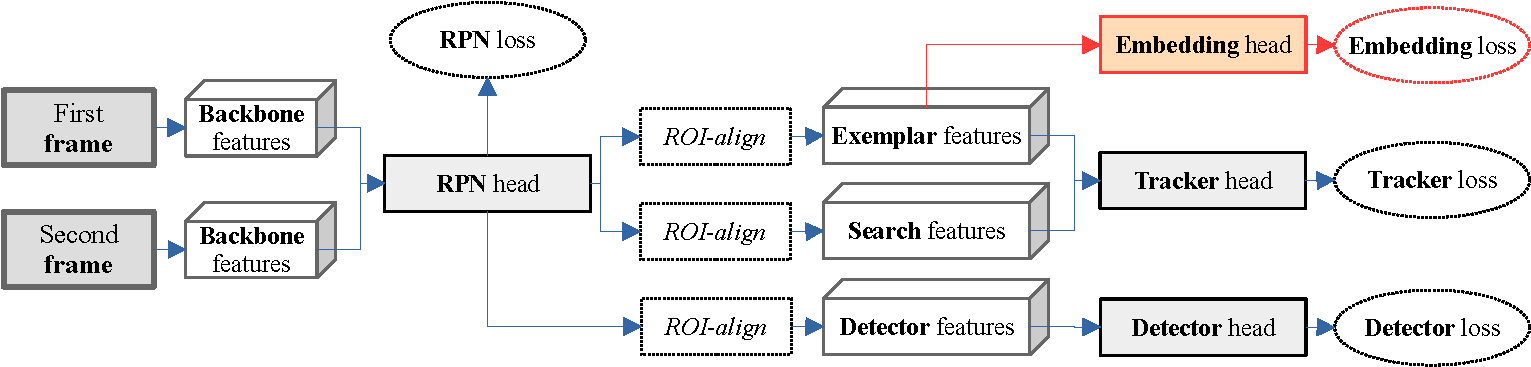
\includegraphics[width=\linewidth]{figures/siamese_tracking/siammot_feature_emb_training.pdf}
    \caption[Embedding-enhanced \gls{siammot} architecture]{Our extension (shown in red) to the underlying \gls{siammot} architecture that incorporates vector embeddings to the end-to-end training. This diagram shows the pipeline that is used during the training, not inference.}
    \label{fig:SiamMOTWithEmbeddings}
\end{figure}
% ------------------------------------------------------------------------------

As far as the vector embedding computation was concerned, we attached the embedding head (\tabletext{}~\ref{tab:FeatureEmbeddingHead}) into the backbone features but after the \gls{roi}-pooling operation (\figtext{}~\ref{fig:SiamMOTWithEmbeddings}). This ensured fixed tensor shapes and allowed us to process the very same features that the object detector and Siamese tracker utilized, too. Simply put, for every proposal made for a particular frame, we looked at the delineated \gls{bbox} through the lens of \gls{roi}-pooling to extract backbone features. In fact, we simply reused the extracted exemplar features. Later on, we processed these features using our newly devised embedding head to produce feature embeddings. The resulting embeddings were subjected to the triplet loss computation (discussed next) with all the necessary operations such as various types of hard negative mining.

\begin{table}[!t]
    \centering
    \begin{tabular}{lll}
        \toprule
        \textbf{layer}    & \textbf{tensor shape}        & \textbf{parameters no.} \\
        \midrule
        input             & $\sbrackets{B, 128, 15, 15}$ & $0$                     \\
        \midrule
        conv $3 \times 3$ & $\sbrackets{B, 128, 13, 13}$ & $147\ 456$              \\
        ReLU              & $\sbrackets{B, 128, 13, 13}$ & $0$                     \\
        \midrule
        conv $3 \times 3$ & $\sbrackets{B, 256, 11, 11}$ & $294\ 912$              \\
        ReLU              & $\sbrackets{B, 256, 11, 11}$ & $0$                     \\
        \midrule
        flatten           & $\sbrackets{B, 30976}$       & $0$                     \\
        linear            & $\sbrackets{B, 1024}$        & $31\ 720\ 448$          \\
        \midrule
        $l_2$-normalize   & $\sbrackets{B, 1024}$        & $0$                     \\
        \bottomrule
                          & \textbf{total}               & $32\ 162\ 816$          \\
        \cline{2-3}
    \end{tabular}
    \caption[Feature embedding head]{Our custom embedding head that we used to process backbone-extracted features to produce embedding vectors. It is built from two convolutional layers separated by a \gls{relu} nonlinearity followed by a fully connected layer which produces a $1024$ dimensional feature embedding. The batch size dimension is given by $B$ in the tensor shape. Since each embedding vector is normalized to unit length, we avoided learning biases throughout the whole network.}
    \label{tab:FeatureEmbeddingHead}
\end{table}

% ##############################################################################
\subsection{Training Phase}

The training phase was altered by adding another loss function to the sum of already existing three losses from the original model. In particular, the general \gls{siammot} loss function defined in \eqtext{}~\ref{eq:SiamMOTGeneralLoss} was reformulated as
\begin{equation}
    \label{eq:SiamMOTFeatureEmbLoss}
    \lossf = l_{rpn} + l_{detect} + l_{motion} + l_{emb}.
\end{equation}
The $l_{emb}$ loss incorporated triplet loss (\eqtext{}~\ref{eq:TripletLoss} on page~\pageref{eq:TripletLoss}). We also experimented with the contrastive loss (\eqtext{}~\ref{eq:ContrastiveLoss} on page~\pageref{eq:ContrastiveLoss}), but the effect was detrimental in every aspect, so we will not discuss it any further. As we remarked in \sectiontext{}~\ref{sec:LatentSpacesAndEmbeddings} on page \pageref{sec:LatentSpacesAndEmbeddings} aimed at latent spaces and embeddings, it is crucial to adopt appropriate sample mining strategies when using the triplet loss. The rationale is that for the training to keep progressing, the model needs to encounter harder and harder triplets to generate sufficient learning signals. To this end, we went for the semi-hard triplet mining strategy (\eqtext{}~\ref{eq:BatchHardMining} on page~\pageref{eq:BatchHardMining}). However, we struggled with collapsing embeddings~\cite{levi2021rethinking}. This phenomenon happens when the embedding training forces the model to project all the features onto a single point in the embedding space, thus incurring the loss equal to the used margin. We claim that the use of semi-hard negative mining produced triplets that were too difficult. Since we used all the \gls{rpn} proposals to generate triplets, one may imagine that there would always be proposals covering only some small part of the object, making it problematic for the network to learn the concept of ``similarity'' and ``difference'' if it only processes very hard images. Nevertheless, these situations are very common in margin-based losses~\cite{levi2021rethinking}. The computed loss is so high that it is more suitable for the model to map all the features onto a single embedding vector. To remedy this, we implemented batch-all online mining strategy (\eqtext{}~\ref{eq:BatchAllLossFunction} on page \pageref{eq:BatchAllLossFunction}), which stabilized the training. We recommend first utilizing batch-all mining strategy during the training, and then slowly proceeding to batch-hard strategy after a certain point. We still have not implemented this approach, because it would be time-consuming to find the right hyperparameters. There are many open questions, such as to mine the \gls{rpn} proposals in a better way or to set the margin to a higher value. Loss functions aimed at object \gls{reid} are notoriously cumbersome to train. One last remark is that we implemented the entire mining algorithm followed by the loss computation in a \gls{gpu}-only fashion for fast execution and easy integration into the pipeline.

% ##############################################################################
\subsection{Inference Phase}

\subsubsection{Feature-based Non-Maximum Suppression}
\label{sssec:FeatureNonMaximumSuppression}

Salscheider~\cite{salscheider2020featurenms} proposed an extended \gls{nms} algorithm that incorporates a distance between feature embeddings dubbed as \featurenms{}. Considering our idea introduced above, we had to encompass the vector embeddings into the solver reasoning. In the beginning, we came up with the solution that exactly copied the one the mentioned author proposed. That provided further justification for attempting to implement the algorithm and test it in practice. The advantage is that this approach is restricted to the inference phase, thus experimenting with it did not require model re-training.

We assume the reader is acquainted with the original \gls{nms} algorithm (more in \sectiontext{}~\ref{ssec:NonMaximumSuppression}.). Nevertheless, here we repeat the same definitions for clarity. Let $\mset{B} = \cbrackets{\vect{b}_1, \vect{b}_2, \dots, \vect{b}_n}$ be a set of $n$ region proposals described by $n$ \glspl{bbox}. Scores for each detection are contained in a set $\mset{S} = \cbrackets{s_1, s_2, \dots, s_n}$, where $s_i$ denotes a detection score for the $i$-th box, $\vect{b_i}$. This time, we are also going to need the associated feature embedding vectors with each \gls{bbox}, represented by a set $\mset{E} = \cbrackets{\vect{e}_1, \vect{e}_2, \dots, \vect{e}_n}$. Let $\mset{B}_{fnms}$ be  the set of filtered proposal instances from the set $\mset{B}$ produced using the \featurenms{} algorithm.

\def\threshlower{\tau_{\text{lower}}}
\def\threshupper{\tau_{\text{upper}}}
\def\threshsim{\delta}

The distinction in terms of parameters is the following. The original algorithm required only one threshold for the maximum allowed portion of the overlap between regions. The \featurenms{} requires three parameters discussed below.
\begin{itemize}
    \item A minimum threshold $\threshlower$ denoting the boundary below which the two objects are deemed as different. This value should be low, for example, $0.2$, which means that if the \gls{iou} between the two objects is less than $0.2$, then the two instances should be treated as different objects.
    \item A maximum threshold $\threshupper$ denoting a boundary above which the two objects are considered to be identical. Conversely to the $\threshlower$, this value should be high, for instance, $0.8$, which indicates that if the \gls{iou} of the two object instances surpasses this threshold, then it should be the same object, and thus, the \gls{bbox} with the lower confidence is discarded.
    \item A threshold $\threshsim$ is used as a decision boundary between the embedding vectors. This threshold should reflect a measure of similarity. If the adopted measure of similarity (cosine distance, Euclidean distance, ...) falls below $\threshsim$, then the two objects are different, otherwise, they are considered the same one. This value of $\threshsim$ is used only if the two conditions above do not hold.
\end{itemize}

Here we provide a pseudocode of the \featurenms{} algorithm:

\begin{algorithmic}[1]
    \Function{Feature-NMS}{$\mset{B}$, $\mset{S}$, $\mset{E}$, $\threshlower$, $\threshupper$, $\threshsim$}

    \State $\mset{B}_{fnms}$ $\gets$ $\emptyset$
    \Comment{initialize the output (filtered) set of region proposals}

    \While {$\mset{B} \neq \emptyset$}
    \Comment{loop until all the proposals are processed}

    \State $m \gets \underset{i \in \cbrackets{1, 2, \dots, \msetsize{S}}}{\argmax{}} \mset{S}$
    \Comment{find an index of a proposal with the highest score}

    \State $\mset{B} \gets \mset{B} - \vect{b}_m$, $\mset{S} \gets \mset{S} - s_m$, $\mset{E} \gets \mset{E} - \vect{e}_m$
    \Comment{remove the proposal}

    \State $\mset{B}_{fnms} \gets \mset{B}_{fnms} \cup \vect{b}_m$
    \Comment{save the proposal with the highest score}

    \For{$i \gets 1$ to $\msetsize{B}$}
    \Comment{iterate through remaining proposals}

    \If{\Call{iou}{$\vect{b}_m$, $\vect{b}_i$} $\geq \threshlower$}
    \Comment{above the lower-bound threshold}

    \If{\Call{iou}{$\vect{b}_m$, $\vect{b}_i$} $\geq \threshupper$}
    \Comment{above the upper-bound threshold}

    \State $\mset{B} \gets \mset{B} - \vect{b}_i$, $\mset{S} \gets \mset{S} - s_i$, $\mset{E} \gets \mset{E} - \vect{e}_i$
    \Comment{remove the proposal}

    \Else

    \If{\Call{similarity}{$\vect{e}_m$, $\vect{e}_i$} $\geq \threshsim$}
    \Comment{similarity above threshold}
    \State $\mset{B} \gets \mset{B} - \vect{b}_i$, $\mset{S} \gets \mset{S} - s_i$, $\mset{E} \gets \mset{E} - \vect{e}_i$
    \Comment{remove the proposal}
    \EndIf

    \EndIf
    \EndIf
    \EndFor
    \EndWhile

    \State \Return $\mset{B}_{fnms}$
    \EndFunction
\end{algorithmic}

% ##############################################################################
\subsection{Experimental Evaluation and Discussion}

The proposed embedding-based enhancement was evaluated against the baseline model without the embedding head. For a fair comparison, we made sure that the hyperparameters were identical to the greatest possible extent. We only had to alter the batch size and learning rate. Since the triplet loss requires the computation of a great number of triplets, especially the batch-all strategy, we had to decrease the batch size to avoid crashes due to not having enough \gls{gpu} \gls{vram} available.

We acknowledge that it is difficult to compare the baseline model with the proposed extension since they progress differently during the training. Therefore, we saved the model state after $K$ training iterations and then evaluated the performance using the validation dataset. The same process was repeated for the baseline architecture, which we trained from scratch using smaller batch sizes. Furthermore, the embedding evaluation also requires the cosine similarity threshold. We tried multiple different values to see the effect.

\todo[inline]{Add ``baseline vs. embedding'' $2$D scatter plot - \gls{mota} vs. \gls{motp}.}
\todo[inline]{Add ``baseline vs. embedding'' $2$D scatter plot - precision vs. recall.}
\todo[inline]{Add a table with quantitative comparison.}
\todo[inline]{Add an ablation study ``\gls{reid} training + original solver'' to see the effect.}

% ##############################################################################
\subsection{Discussion}

We conjecture that our inability to improve the tracker performance was caused by the introduction of the feature embedding itself, as it was the only change during the training phase. Our ablation study also demonstrated that joint training with the embedding head had a negative impact on the tracker, even if the original solver was adopted during the evaluation. This raises the question of potential task/feature conflict between the heads. We venture to claim the inherent incompatibility of the detection, tracking, and \gls{reid} tasks, despite the existence of a recently published work Lu~\etal{}~\cite{lu2020retinatrack}, who developed their \retinatrack{} tracker. This framework exploited the base visual object detector called a \retinanet{}~\cite{lin2018focal} and then added, in principle, a very similar head as we did for the purpose of producing feature embeddings. However, there are obvious differences between the two trackers in terms of how the inference phase is executed, and that is where we see one of the possible causes of our failure.

\subsubsection{Unfairness between the detection and re-identification}

There is a recent publication~\cite{zhang2021fairmot} by Zhang~\etal{} that discusses the notion of ``fairness'' between detection and \gls{reid}. According to their empirical evidence, there are multiple levels in which the ``unfairness'' manifests itself. This term was used to describe a situation in which the importance of either \gls{reid} or detection task is lessened. We would like to emphasize the recency of this work since several of their remarks and conclusions coincide with ours. Had we encountered this paper prior to conducting our experiments, we would have taken a different path. At least, we would have striven to find another way to incorporate the embedding creation into an end-to-end pipeline. The aforementioned work, among other things, introduces a joint tracker that effectively circumvents the obstacles related to conflicting tasks. This framework avoids the use of anchor proposals and is based on \gls{centernet}~\cite{zhou2019centernet} object detector.

They argue that the \gls{reid} task may become overlooked if the embedding vectors are produced solely from the \gls{roi}-pooled regions, as in our case. Consequently, the detection task becomes central in terms of influence upon the loss function since generating embedding vectors on incorrect \glspl{bbox} is meaningless. Thus, the bias to produce accurate object proposals is inescapable.

Next, a problem arises when one anchor corresponds to multiple identities, which is an obstacle we have already mentioned. As a result, the extracted features are not optimal in terms of their accuracy as well as discriminative representativeness. To remedy this, features should be extracted at a single point, \ietext{}, at the estimated object centers (hence the use of \gls{centernet}), instead of region proposals.

An analogical problem is when multiple anchors correspond to one identity. A high overlap in terms of \gls{iou} directs the model to estimate the same identity for nearby anchors. But, even small perturbation may result in falling below a specific threshold and the anchors become marked as belonging to different objects. In fact, this situation is very common as proposals are generated on the feature level (a coarse representation due to downsampling), and not the pixel level.

Another inherent problem when merging object detection and \gls{reid} is feature conflict. We have highlighted numerous times the significance of multi-layer feature fusion. However, not all tasks benefit from this approach equally. In particular, object detection utilizes deep features to estimate object classes and locations, whereas the \gls{reid} is more prone to utilizing low-level features owing to their discriminative power. For that reason, it is important to balance the loss optimization.

And last but not least, the feature dimension poses another source of imbalance. The authors remarked that actually learning lower-dimensional features for \gls{reid} is better than higher-dimensional. In our research, we thought the opposite is true. High-dimensional embedding vectors notably harm the object detection accuracy due to the competition between the two tasks. The number of feature dimensions for detection is usually very low (compared to $1024$D or $2048$D embedding vectors). We adopted high-dimensional vector embeddings in conjunction with the usual low-dimensional detector features, thus exacerbating the rivalry between the two. The rationale behind proposing to use, \egtext{}, $64$D embedding vectors, is that the \gls{mot} task performs just a few one-to-one matchings between two consecutive frames. However, there is a tacit assumption of having all objects sufficiently visible, as this work did not cover occlusion handling and their benchmark evaluations were not specifically targeted at full object occlusion. This is a path definitely worth exploring. Nonetheless, the proposed framework achieved \gls{sota} performance among \gls{mot} approaches, surpassing the competitive frameworks by a large margin even in terms of \gls{fps}.

\section{Siamese Multi-Object Tracking and Attention}
\label{sec:SiamMOTandAttention}

% ##############################################################################
\subsection{Motivation}

During several evaluation runs and our manual inspection of the tracker performance, we noticed a ubiquitous pattern. We remind that the scenes on which we trained as well as tested our tracker were captured by a static camera. Consequently, several video sequences contained multiple vehicles standing still, due to a traffic jam or an ongoing red light, but viewed under an angle somewhere in the range of $30-60$ degrees (\figtext{}~\ref{fig:UADETRACPartialOcclusion}). Therefore, it resulted in a partial occlusion. However, what we considered even more problematic was the inability of the axis-aligned \gls{bbox} to properly define the vehicle as the angle under which the car was visible caused the \gls{bbox} to capture a great portion of the neighboring vehicles even without severe occlusion happening.

% ------------------------------------------------------------------------------
\begin{figure}[!t]
    \centerline{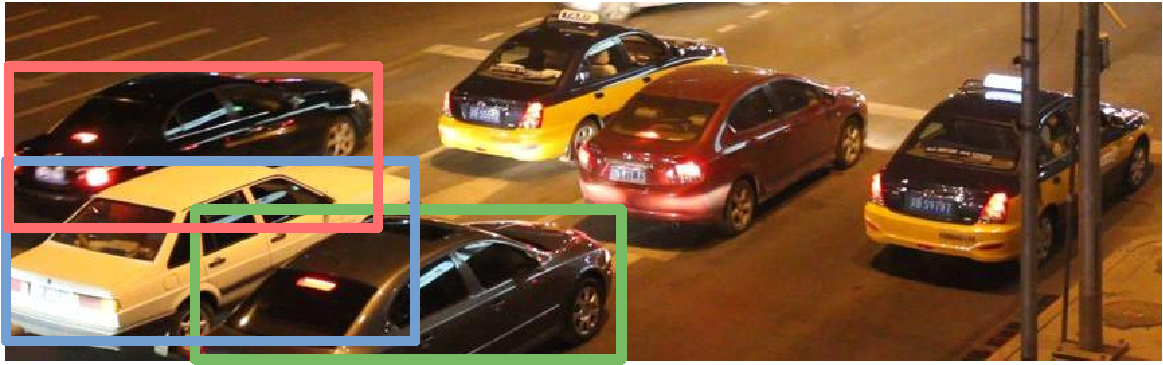
\includegraphics[width=0.7\linewidth]{figures/siamese_tracking/uadetrac_partial_occlusion_red_light.pdf}}
    \caption[Partial occlusion in the \uadetrac{} dataset]{An example of a situation where multiple vehicles are standing still on a cross-road. In this scenario, even though just a slight degree of occlusion is present, the biggest issues are caused by the need to delineate \glspl{roi} using axis-aligned \glspl{bbox}. This inevitably captures the neighboring vehicles, increasing the likelihood of drifting to semantic background due to presence of similar interference, \ietext{}, distractors.}
    \label{fig:UADETRACPartialOcclusion}
\end{figure}
% ------------------------------------------------------------------------------

Situations described above reminded us of the \gls{siammask}~\cite{wang2019siammask} single object tracker targeted at predicting segmentation mask along with the usual single-object Siamese tracking routine. Such prediction was subsequently exploited to produce a rotated \gls{bbox} instead of an axis-aligned one. Even though the evaluation benchmarks only consider axis-aligned predictions, the rotated region served the purpose of enhancing the discriminative power of the tracker, primarily when dealing with occlusion. In the scenario shown in \figtext{}~\ref{fig:UADETRACPartialOcclusion}, a rotated \gls{bbox} would inexorably lead to an improved tracking accuracy. This approach was deemed successful for general object tracking, thus it also spawned another follow-up work of \gls{siammaske}~\cite{chen2019rotbboxes} which altered the original formulation of predicting the rotated \gls{bbox} by use of ellipse fitting for even better accuracy.

However, there is a lack of datasets providing rotated annotations. The \uadetrac{} dataset is no exception. As a result, we sidestepped this approach and searched for an alternative solution that would enhance the discriminative power of the tracker when faced with partial occlusion. One such approach was the use of attention~\cite{vaswani2017attention}, especially spatial attention, which we found effective during our survey research~\cite{ondrasovic2021siamese}. Apart from the attention mechanism, we also remembered the more general formulation of the convolution operation, which has been shown to significantly better object detection tasks due to the semi-dense prediction requirements, dubbed as deformable convolution~\cite{dai2017dcnn}. In what follows, we will discuss these two methods (\sectiontext{}~\ref{ssec:Attention} and \sectiontext{}~\ref{ssec:DeformableCNNs}) as a foundation for our subsequent experiments that yielded a positive outcome.

% ##############################################################################
\subsection{Attention}
\label{ssec:Attention}

An attention mechanism was first introduced by Vaswani~\etal{}~\cite{vaswani2017attention}. The use of encoder-decoder architectures to capture a complete sequence of information by a single vector spurred the development of the attention module. This use case poses problems in holding on to information at the beginning of the sequence and encoding long-range dependencies. To address this, the attention module computes attentions, or, in other words, the degree of relevance between ``queries'' and ``keys'', to retrieve ``values'' in adequate proportions.

The concept of ``queries, keys and values'' comes from information retrieval systems. Let us provide a demonstrative example based on a YouTube video search. Assume a specific query signaling the demand to retrieve a particular YouTube video. The system then maps this query against a set of keys represented by various features, \egtext{}, video title, description, upload time, etc. These keys are directly associated with the stored candidate videos within the database. The output of this operation is a set of values, \ietext{}, found videos, that best match the given query.

The attention aims to exploit deep learning to learn a transformation of the input (not necessarily the same) into three separate vector spaces, each of them dedicated to a different purpose. The first space is to capture the query, therefore, it should represent features that best describe the query to facilitate information retrieval. The obvious compatriot is the key vector space which is trained to represent the value in the most accurate way to initiate the search accurately. Last but not least, the value vector space extracts features that are most useful for the task at hand. They do not need to capture features pertinent to the search. For that, there are the two other mappings.

For a more concrete demonstration, we will use a scaled dot-product attention. The input consists of queries and keys of dimension $d_k$, and values of dimension $d_v$. The query is used to compute a dot product with all the keys. These computations are scaled by $\sqrt{d_k}$ to provide a temperature scaling for the following softmax transformation to obtain the weights that will be used to retrieve values (\figtext{}~\ref{fig:ScaledDotProductAttention}). For optimal performance, it is reasonable to compute the attention function for the set of queries simultaneously as they can be easily stored in a matrix, denoted by $\mtx{Q}$. Analogically, keys and values can be also packed together into matrices given by $\mtx{K}$ and $\mtx{V}$, respectively. Thus, the attention can be formulated as a function of queries, keys and values, and is defined as
\begin{equation}
    \label{eq:ScaledDotProductAttention}
    \func{attention}{\mtx{Q}, \mtx{K}, \mtx{V}} =
    \func{softmax}{\frac{\mtx{Q} \mtx{K}^T}{\sqrt{d_k}}} \mtx{V}.
\end{equation}

% ------------------------------------------------------------------------------
\begin{figure}[!t]
    \centerline{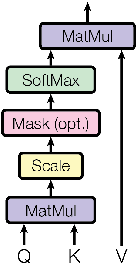
\includegraphics[width=0.15\linewidth]{figures/siamese_tracking/scaled_dot_product_attention.pdf}}
    \caption[Scaled dot-product attention]{An example of the input transformation by the scaled dot-product attention module. The pair of queries and keys is used to produce the probability distribution over the individual values for the final weighted sum. \externalsrc{\cite{vaswani2017attention}}}
    \label{fig:ScaledDotProductAttention}
\end{figure}
% ------------------------------------------------------------------------------

The two most prominent variants of attention are the additive attention~\cite{bahdanau2016additiveattention} and the multiplicative (dot-product) attention, with the latter being identical to the one described above except for the temperature scaling. Just for the record, we experimented with both approaches and we observed differences in performance. On balance, both attentions are similar in theory, however, dot-product is much faster and more space-efficient in practice. On the other hand, additive attention outperforms the dot-product attention as long as temperature scaling is not employed for larger values of $d_k$, since the dot-products tend to push the softmax function to regions of extremely small gradients.

In our work, we also exploited the notion of self-attention. Since attention was first targeted at natural language translation, let us provide an example from this area. Originally, the attention was computed between the input and output sentences. Regarding self-attention, attention is computed with respect to the sentence itself. In terms of computer vision, the spatial self-attention represents a weight map over a $2$D feature map indicating how important each feature element for the particular task is. Analogically, the channel self-attention may be used to attribute importance to individual channels, as they often are not equally important. Moreover, it yields more interpretable models as a by-product~\cite{vaswani2017attention}. These ideas will be explored later.

% ##############################################################################
\subsection{Deformable Convolutional Neural Networks}
\label{ssec:DeformableCNNs}

\Glspl{dcnn}~\cite{dai2017dcnn} are gaining popularity and are being applied to numerous sophisticated computer vision tasks, \egtext{}, object segmentation (dense predictions) and object detection (semi-dense predictions). Since object tracking revolves around the same requirements in terms of pixel-wise precision, we contemplated using this advancement, too.

Although \glspl{cnn} (\sectiontext{}~\ref{ssec:ConvolutionalNeuralNetworks} on page~\pageref{ssec:ConvolutionalNeuralNetworks}) are an excellent tool for a plethora of deep learning tasks involving image processing, they are still limited in their capabilities to model a broad range geometric transformation. To address this, practitioners apply a broad range of data augmentation techniques (\egtext{}, rotation, translation, scaling, shearing, and cropping) to provide the necessary samples of some particular transformation during the training. However, such an approach is limited to tailor-made transformations that may not cover the entire set of possibilities the model may face at test time.

The first work to learn spatial transformation from the training data in a deep learning fashion is known under the name \glspl{stn}~\cite{jaderberg2016stn}. It warps the feature map via a global parametric transformation such as affine transformation. In the realm of convolutional operations, there is the atrous convolution operation~\cite{holschneider1990atrousconv} that enhances the standard convolution by expanding the receptive field while maintaining the same number of parameters by use of greater offsets. However, these offsets are fixed. An obvious successor of this approach is the active convolution~\cite{jeon2017activeconv} that treats convolution offsets as learnable parameters instead of constants. But, in this setting, the learned offsets are shared across different spatial locations. Thus, the most general approach is to determine the offsets at each location independently and then proceed as usual. This is where deformable convolution (\figtext{}~\ref{fig:StandardVsDeformableCNN}) comes into place.

In concrete terms, a $2$D convolution consists of sampling using a regular offset grid $\mset{R}$ defining the receptive field as well as dilation over the input features $\vect{x}$ followed by the summation of the samples values weighted by $\vect{w}$. For example, a standard $3 \times 3$ convolution with dilation $1$ would employ offsets given by
\begin{equation}
    \label{eq:StandardConvolutionOffsetGrid}
    \mset{R} = \cbrackets{
        \rbrackets{-1, -1}, \rbrackets{-1, 0}, \dots, \rbrackets{0, 1}, \rbrackets{1, 1}
    }.
\end{equation}
Then, for each location $\vect{p}_0$ within the output feature map $\vect{y}$ is calculated as
\begin{equation}
    \label{eq:StandardConvolutionOutputCalc}
    \func{\vect{y}}{\vect{p}_0} =
    \sum_{\forall \vect{p}_n \in \mset{R}}
    \func{\vect{w}}{\vect{p}_n} \cdot \func{\vect{x}}{\vect{p}_0 + \vect{p}_n},
\end{equation}
where the locations in $\mset{R}$ are iterated over by $\vect{p}_n$. Conversely, the deformable convolution extends the standard one by augmenting the original sampling grid $\mset{R}$ with additional offsets $\cbrackets{\Delta \vect{p}_n \ |\ n = 1, \dots, \msetsize{R}}$ (\figtext{}~\ref{fig:DeformableCNN}). Thus, \eqtext{}~\ref{eq:StandardConvolutionOutputCalc} is reformulated as
\begin{equation}
    \label{eq:DeformableConvolutionOutputCalc}
    \func{\vect{y}}{\vect{p}_0} =
    \sum_{\forall \vect{p}_n \in \mset{R}}
    \func{\vect{w}}{\vect{p}_n} \cdot \func{\vect{x}}{\vect{p}_0 + \vect{p}_n + \Delta \vect{p}_n}.
\end{equation}
Nonetheless, the user needs to keep in mind that the sampling offsets now become fractions and thus have to be handled accordingly. One approach is to employ bilinear interpolation, where the position in the input feature map $\vect{x}$ is determined by
\begin{equation}
    \label{eq:DeformableConvolutionBilinear}
    \func{\vect{x}}{\vect{p}} =
    \sum_{\forall \vect{q}} \func{G}{\vect{q}, \vect{p}} \cdot \func{\vect{x}}{\vect{p}},
\end{equation}
in which $\vect{q}$ enumerates all integral locations and $\func{G}{\cdot}$ represents the  interpolation kernel. The interpolation processing can be efficiently implemented owing to the sparsity. The performance overhead is negligible compared to the reaped benefits of adaptive sampling locations capable of covering very complicated transformations (\figtext{}~\ref{fig:SamplingLocationsDeformableCNN}).

% ------------------------------------------------------------------------------
\begin{figure}[t]
    \centerline{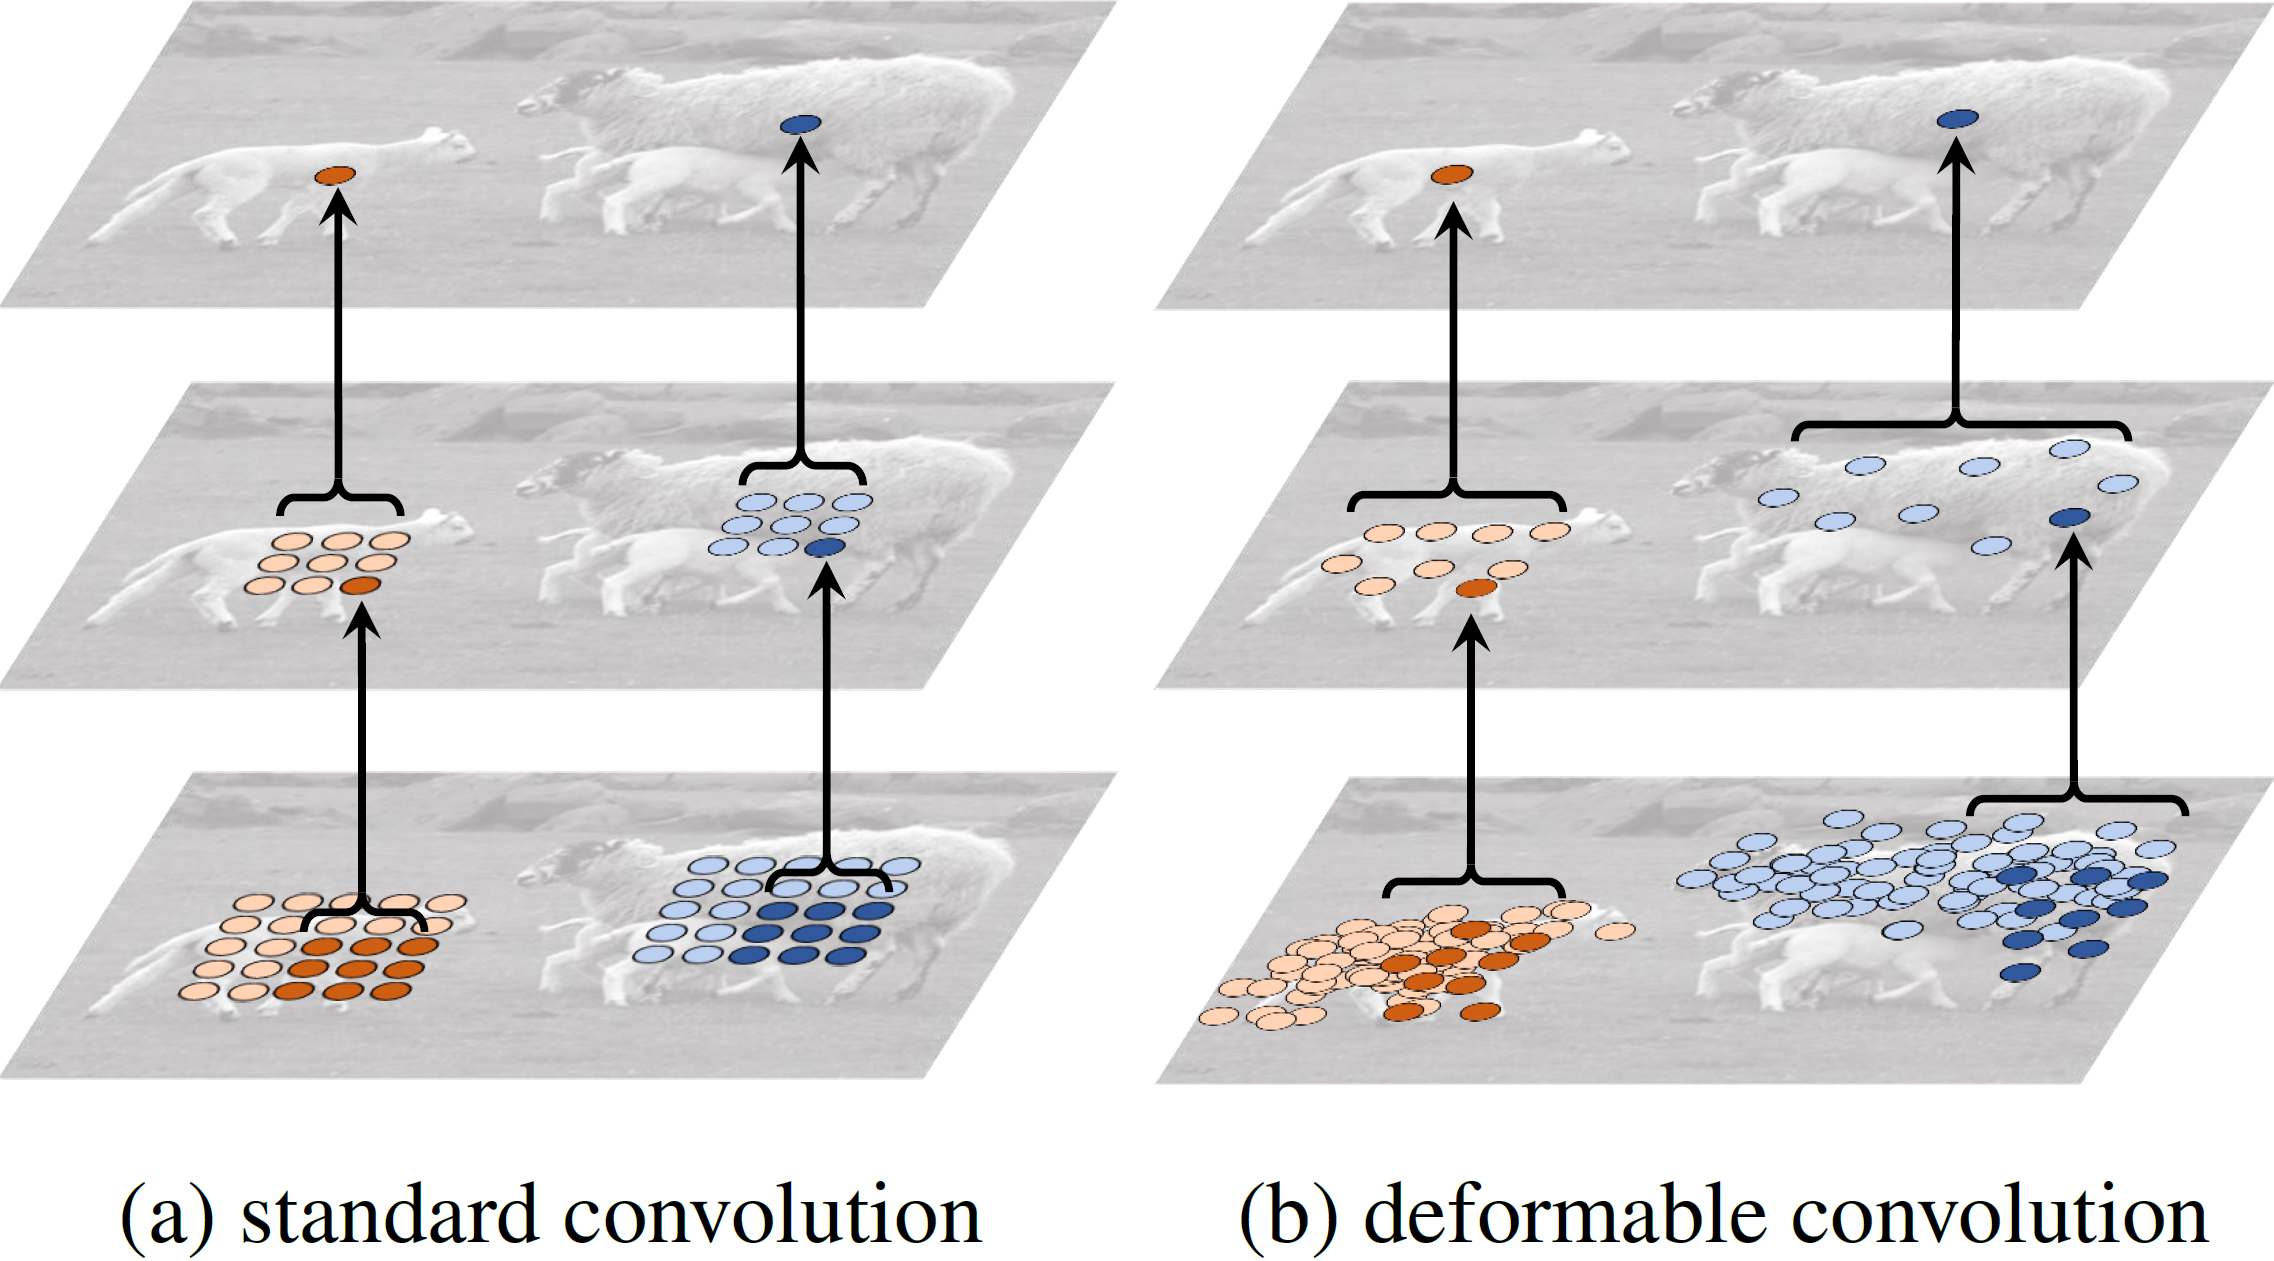
\includegraphics[width=0.6\linewidth]{figures/siamese_tracking/dcn_standard_vs_deformable.png}}
    \caption[Standard vs. deformable convolution]{Visualization of the difference between the fixed \imgpartdesc{a} and adaptive \imgpartdesc{b} receptive fields. Stacking multiple deformable convolutions results in profound amplification of deformation, making the transformation capture diverse shapes that would otherwise be very coarsely approximated by a standard convolution. \externalsrc{\cite{dai2017dcnn}}}
    \label{fig:StandardVsDeformableCNN}
\end{figure}
% ------------------------------------------------------------------------------

% ------------------------------------------------------------------------------
\begin{figure}[t]
    \centerline{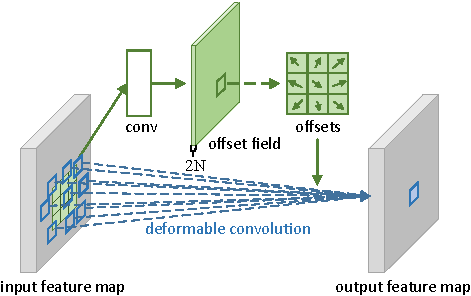
\includegraphics[width=0.6\linewidth]{figures/siamese_tracking/deformable_convolution.pdf}}
    \caption[\Gls{dcnn}]{Illustration of a $3 \times 3$ deformable convolution operation. Unlike the standard convolution operation used in neural networks, this one employs one additional step of predicting variable offsets instead of using a fixed rectangular grid. \externalsrc{\cite{dai2017dcnn}}}
    \label{fig:DeformableCNN}
\end{figure}
% ------------------------------------------------------------------------------

% ------------------------------------------------------------------------------
\begin{figure}[t]
    \centerline{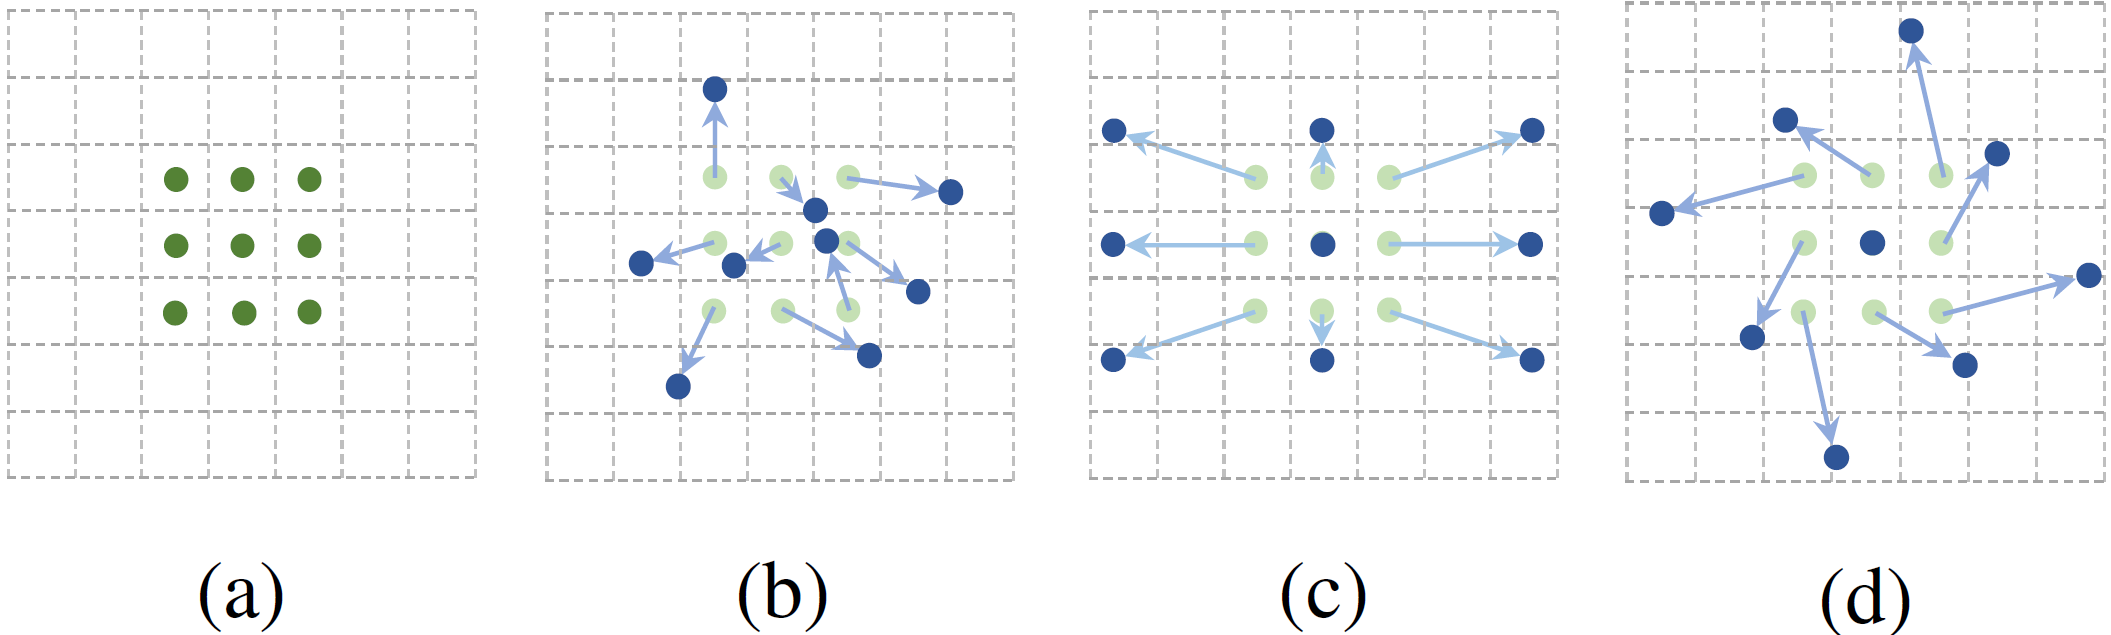
\includegraphics[width=0.7\linewidth]{figures/siamese_tracking/dcn_sampling_locations.png}}
    \caption[Various sampling locations in \glspl{dcnn}]{Deformable convolution is effective at learning appropriate sampling locations reflecting the underlying transformation. \imgpartdesc{a} shows the regular sampling grid of a standard convolution; \imgpartdesc{b} is an example of irregularly deformed sampling region; \imgpartdesc{c} and \imgpartdesc{d} represent an expected pattern corresponding to scaling and rotation operations, respectively. \externalsrc{\cite{dai2017dcnn}}}
    \label{fig:SamplingLocationsDeformableCNN}
\end{figure}
% ------------------------------------------------------------------------------

The original paper~\cite{dai2017dcnn}, in which \glspl{dcnn} were introduced, showed that learning dense spatial transformation in using deep learning by use of \glspl{cnn} or sophisticated vision tasks such as object detection and semantic segmentation is feasible as well as effective. After our experience, we add that object tracking may benefit from this extension, too.

\subsection{Modulated Deformable Convolutional Neural Networks}
\label{ssec:ModulatedDeformableCNNs}

The original paper by Zhu~\etal{}~\cite{zhu2018mdcnn} aptly described their contribution in the headline that contained the words ``more deformable, better results''. Because of this, we will provide a concise description of the \glspl{mdcnn}, an extension to the previously discussed \glspl{dcnn}.

Since we are simply adding a slight modifications to an already introduced equation, we will try to avoid repetition. Thus, let $\vect{p}_0$, $\vect{p}_n$ and $\Delta \vect{p}_n$ have the same meaning as in \eqtext{}~\ref{eq:DeformableConvolutionOutputCalc}. Then, the modified equation becomes
\begin{equation}
    \label{eq:ModulatedDeformableConvolutionOutputCalc}
    \func{\vect{y}}{\vect{p}_0} =
    \sum_{\forall \vect{p}_n \in \mset{R}}
    \func{\vect{w}}{\vect{p}_n} \cdot \func{\vect{x}}{\vect{p}_0 + \vect{p}_n + \Delta \vect{p}_n} \cdot \Delta \vect{m}_n,
\end{equation}
where $\Delta \vect{m}_n$ is the modulation scalar for the current location, such that $\Delta \vect{m}_n \in \rbrackets{0, 1}$. Thus, there are two types of learnable parameters. The already described offsets, given by the $\Delta \vect{p}_n$ term, and the new modulation (weighting) coefficients, represented by the term $\Delta \vect{m}_n$. This trivial extension allows the system to not only learn how to sample features in a non-regular fashion if needed, but it also allows applying distinct weight to each sampling location to further adaptively intensify the deforming effect. Although the weights of the underlying convolutional layer can be tweaked to a large extent in order to apply different weights to different features, the inclusion of additional weighting coefficient provides more \glspl{dof}.

From an implementation standpoint, \glspl{dcnn} as well as \glspl{mdcnn} have learnable offsets (and modulation coefficients, if used) set to zero during initialization. This produces no deformable effect, so the convolution behaves as usual in terms of location sampling. However, the modulation aspect is slightly different. Since the sigmoid function is commonly adopted to project the modulation weights into the $\rbrackets{0, 1}$ interval, it multiplies each location by the value of $\func{sigmoid}{0} = \nicefrac{1}{2}$ at the beginning.

% ##############################################################################
\subsection{Deformable Siamese Attention}
\label{ssec:DeformableSiameseAttention}

The two independent ideas above led us to experiment with a self-attention mechanism aimed at enhancing feature selection in both spatial and channel domain. Such experiments resulted in slight improvements for the reasons outlined in the motivation section. To support that our ideas were based on properly identified causes, there is a recently published work demonstrating the effectiveness of the very same approach.

Yu~\etal{}~\cite{yu2021dsa} formulated their \gls{dsa}, which covered both of our suggestions above and additionally introduced the notion of cross-attention as an enhancement to the self-attention itself. What primarily motivated the introduction of the cross-attention was that the exemplar and search region features in Siamese trackers are computed separately, yet they may frequently compensate each other. It is reasonable to assume that multiple objects appear at the same time even in \gls{sot}, let alone \gls{mot}. Consequently, it is of paramount importance for the search branch to have as much information as possible about the exemplar during the computation of the response map for better discrimination. By the same token, the exemplar features may be enhanced by information from the search features. To this end, the cross-attention, at the acceptable computational cost, serves properly in a predictable fashion.

% ------------------------------------------------------------------------------
\begin{figure}[t]
    \centerline{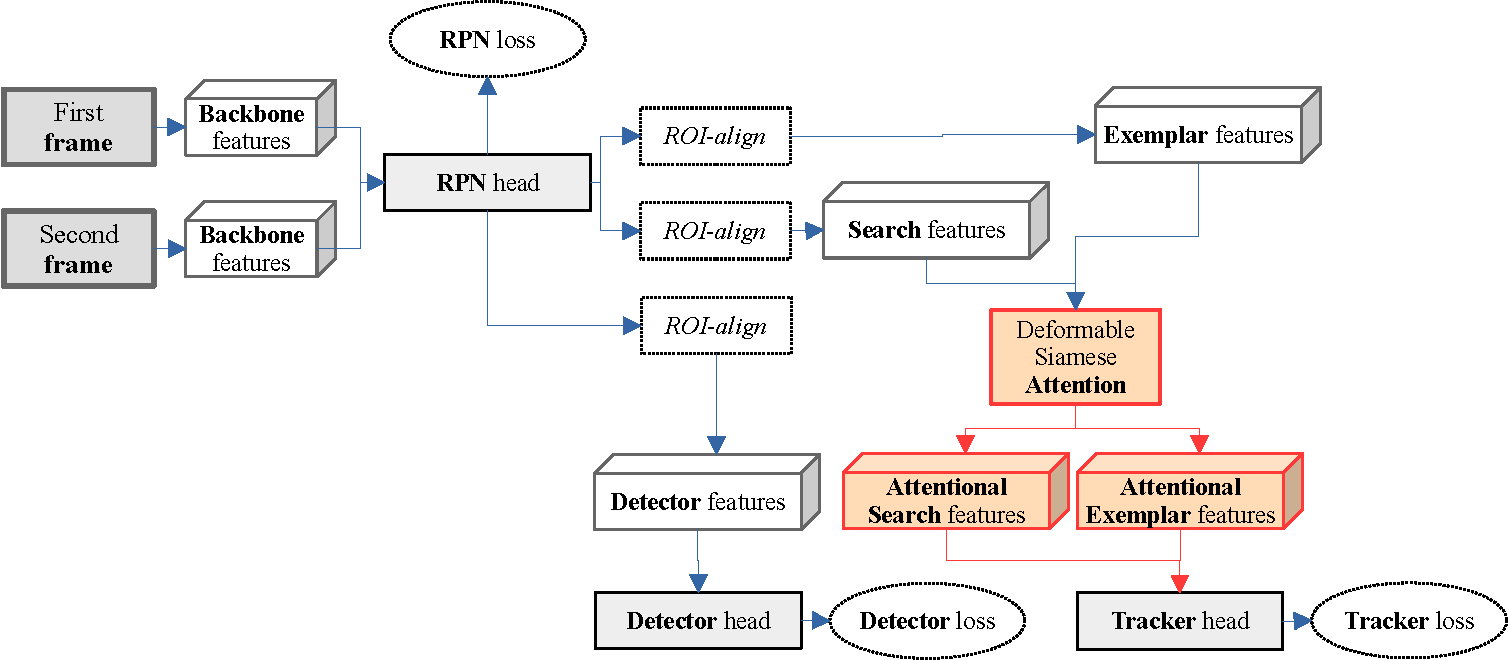
\includegraphics[width=\linewidth]{figures/siamese_tracking/siammot_attention_training.pdf}}
    \caption[\Gls{siammot} with attention]{Our proposal to incorporate attention into the \gls{siammot} pipeline. This diagram shows the relationships between individual parts of the framework during the training phase.}
    \label{fig:SiamMOTWithAttention}
\end{figure}
% ------------------------------------------------------------------------------

Considering their contribution and promising outcomes for the \gls{sot} demonstrated on the \gls{siamrpn} framework (\sectiontext{}~\ref{ssec:TrackingUsingSiameseNetworks} on page \pageref{ssec:TrackingUsingSiameseNetworks}), we decided to implement their proposed module into the \gls{siammot} tracker as described in their paper (\figtext{}~\ref{fig:SiamMOTWithAttention}). However, with the prospect of greater improvement, we adopted modulated \glspl{dcnn}, instead of pure \glspl{dcnn}, because the \Glspl{mdcnn} have all the advantages of the standard deformable convolution, but they additionally learn a modulation (weighting) for individual elements of the feature map while taking the underlying features into account. For our purposes, this seemed to intensify the spatial attention effect, since not only the deformable part was responsible for choosing features using irregular sampling patterns, the network was even allowed to weigh them differently. We conjectured that such an extension may either have no dramatic effect or influence it only positively.

% ------------------------------------------------------------------------------
\begin{figure}[t]
    \centerline{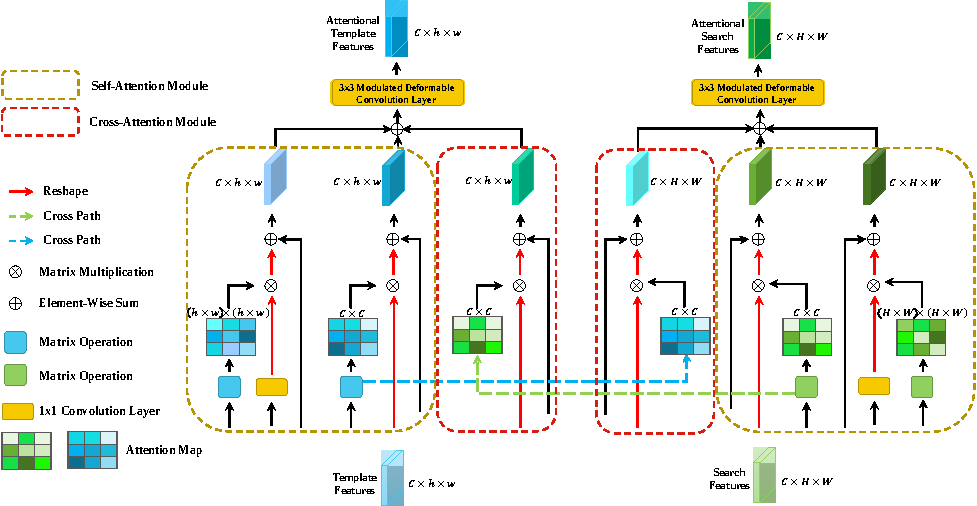
\includegraphics[width=\linewidth]{figures/siamese_tracking/deformable_siamese_attention.pdf}}
    \caption[\Gls{dsa} diagram]{The \gls{dsa} extension introduces two sub-modules for both exemplar and search branch. The self-attention is further divided into two operations, namely the spatial and channel attention. The very same attention network is used to process both features independently. Notice how the channel attention is computed only once as part of the self-attention process and then directly fused with the channel self-attention of the other branch, creating the cross-attention effect, which is the strongest one from all three, according to authors. \externalsrc{\cite{yu2021dsa}}}
    \label{fig:DeformableSiameseAttention}
\end{figure}
% ------------------------------------------------------------------------------

\subsubsection{Self-Attention}

Self-attention is computed separately on the exemplar and search branch independently. This operation can be easily achieved since exemplar and search tensors only differ in width and height. The following description of the self-attention computation conforms to the established attention principles regarding ``queries, keys and values'' introduced in \sectiontext{}~\ref{ssec:Attention}. For better understanding of the computation, see the diagram in \figtext{}~\ref{fig:DeformableSiameseAttention}.

Let $\mtx{X} \in \setrnnn{C}{H}{W}$ be the input features. To produce query features $\mtx{Q}$ and key features $\mtx{K}$, such that $\mtx{Q}, \mtx{K} \in \setrnnn{C^{\prime}} {H}{W}$ and $C^{\prime} = \frac{1}{4}C$, where $C^{\prime}$ is the reduced number of channels, two separate $1 \times 1$ convolution layers are applied. The two obtained features then need to be reshaped into $\mtx{\bar{Q}}, \mtx{\bar{K}} \in \setrnn{C^{\prime}}{N}$, where $N = H \times W$. The spatial self-attention $\mtxsubsup{A}{S}{S} \in \setrnn{N}{N}$ is then produced via matrix multiplication and a column-wise softmax operation as
\begin{equation}
    \label{eq:SpatialSelfAttention}
    \mtxsubsup{A}{S}{S} =
    \func{softmax_{col}}{\mtx{\bar{Q}}^T \mtx{\bar{K}}}.
\end{equation}
Authors used $C^{\prime} = \frac{1}{8}C$, but in \gls{mot}, the number of objects to track is often a lot greater, thus the computation graph grows dramatically with the higher number of channels. Furthermore, in our case $C = 128$, and we considered using $32$ channels for the attention to be the bare minimum.

Meanwhile, an analogous sequence of operations is adopted to produce the value features. A $1 \times 1$ convolution layer without the subsequent reshape operation transforms the input features $\mtx{X}$ into the value features $\mtx{\bar{V}} \in \setrnn{C}{N}$. At this point, we have matched the queries with keys and computed the values. We may proceeed further to the weighted selection from the values and to incorporate the attention into the features as follows
\begin{equation}
    \label{eq:SpatialSelfAttentionApplication}
    \mtxsubsup{\bar{X}}{S}{S} =
    \alpha \mtx{\bar{V}} \mtxsubsup{A}{S}{S} + \mtx{\bar{X}},
\end{equation}
where $\alpha$ is a learnable scalar parameter, and $\mtxsubsup{\bar{X}}{S}{S} \in \setrnn{C}{N}$. The outputs $\mtxsubsup{\bar{X}}{S}{S}$ are then reshaped back to the original size, specifically $\mtxsubsup{X}{S}{S} \in \setrnnn{C}{H}{W}$. From our experience, the parameter $\alpha$ is very useful for training stabilization.

The corresponding channel self-attention $\mtxsubsup{A}{C}{S}$ and the channel-wise attentional features $\mtxsubsup{X}{C}{S}$ are obtained similarly. Due to space limitations and the fact that the upcoming formulation of the cross-attention exploits the channel self-attention, we will omit a detailed description. We will just point out that the ``queries, keys and values'' for the channel self-attention are produced directly from the features on the input, with no $1 \times 1$ convolutions whatsoever. The final self-attentional features are generated by an element-wise sum using the partial spatial and channel self-attentions, $\mtxsubsup{X}{S}{S}$ and $\mtxsubsup{X}{C}{S}$, respectively.

\subsubsection{Cross-Attention}

Let $\mtx{Z} \in \setrnnn{C}{h}{w}$, $\mtx{X} \in \setrnnn{C}{H}{W}$ denote the exemplar and search region features, respectively. The following description introduces the computation of the cross-attention from the perspective of the search branch. First, the exemplar features $\mtx{Z}$ are reshaped into $\mtx{\bar{Z}} \in \setrnn{C}{n}$, where $n = h \times w$. Then, the cross-attention from the exemplar branch is computed. We emphasize that the channel attention is reused, therefore, the computation below serves as a recipe for how to compute the channel self-attention. So, we compute the channel cross-attention $\mtxsup{A}{C} \in \setrnn{C}{C}$ as
\begin{equation}
    \label{eq:CrossAttentionCalc}
    \mtxsup{A}{C} =
    \func{softmax_{row}}{\mtx{\bar{Z}} \mtx{\bar{Z}}^T}.
\end{equation}
The real benefit comes from the merging stage, where the above-computed attention is merged with the other, in this case, the search branch as
\begin{equation}
    \label{eq:CrossAttentionMerge}
    \mtxsup{\bar{X}}{C} =
    \gamma \mtxsup{A}{C} \mtx{\bar{X}} + \mtx{\bar{X}},
\end{equation}
where $\gamma$ is a learnable scalar parameter. The merged features $\mtxsup{\bar{X}}{C}$, once again, have to be reshaped, so the features $\mtxsup{X}{C} \in \setrnnn{C}{H}{W}$ are the final output.

At last, the self-attentional features are combined with the cross-attentional features using element-wise sum. The cross-attention from the perspective of the exemplar branch can be obtained using a similar sequence of operations. In total, there are six steps that involve addition for the purpose of feature merging (\figtext{}~\ref{fig:DeformableSiameseAttention}).

Once the attention is applied to tracking, the corresponding response map is altered as expected. Discriminative power of the tracker is enhanced by appropriate suppression of the semantic background. As \figtext{}~\ref{fig:DSAAttentionVisualization} shows, activations in the search regions as viewed through the response map vary if the \gls{dsa} module is included in the computation, making the tracker less prone to drifting to scene or semantic background objects.

\subsubsection{Deformable Convolution Phase}

The attention is finalized by processing the obtained feature tensors by another layer of modulated deformable convolution. We modified the deformable convolution operation to include the modulated version, which is our modification compared to the original formulation (\figtext{}~\ref{fig:DeformableSiameseAttention}, top yellow boxes). The resulting features with shape identical to the input shape are used to compute the response map. As a result, this extension can be easily integrated into an existing pipeline thanks to its ability to preserve tensor shapes.

% ------------------------------------------------------------------------------
\begin{figure}[t]
    \centerline{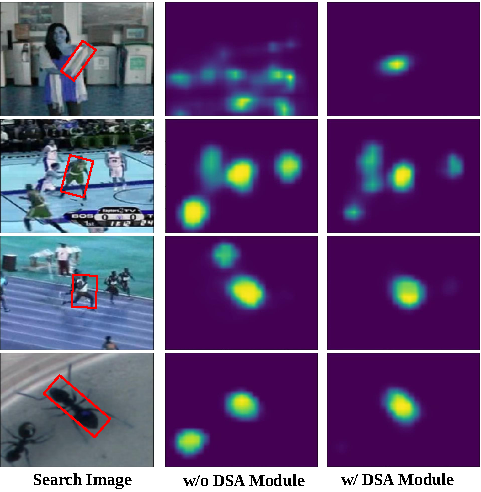
\includegraphics[width=0.5\linewidth]{figures/siamese_tracking/dsa_attention_visualization.pdf}}
    \caption[\Gls{dsa} attention visualization]{Visualization of response (confidence) maps. The first column represents the search image, the second column represents the activation levels without the \gls{dsa} module, whereas the third column clearly demonstrates the improved target-background discirminability in the computed attentional features. \externalsrc{\cite{yu2021dsa}}}
    \label{fig:DSAAttentionVisualization}
\end{figure}
% ------------------------------------------------------------------------------

% ##############################################################################
\subsection{Experimental Evaluation}
\label{ssec:DSAExperimentalEvaluation}

\todo[inline]{Add experimental evaluation. Don't forget about gradient accumulation.}

% ##############################################################################
\subsection{Discussion}
\label{ssec:DSADiscussion}

\todo[inline]{Add discussion.}

